% 例 2（直角存在性）：A(0,3), B(4,0)，C 在 x 轴；2 解 C1(0,0), C2(-9/4,0)
\documentclass[tikz,border=4pt]{standalone}
\usepackage{ctex}
\usepackage{amsmath}
\usetikzlibrary{calc}
\begin{document}
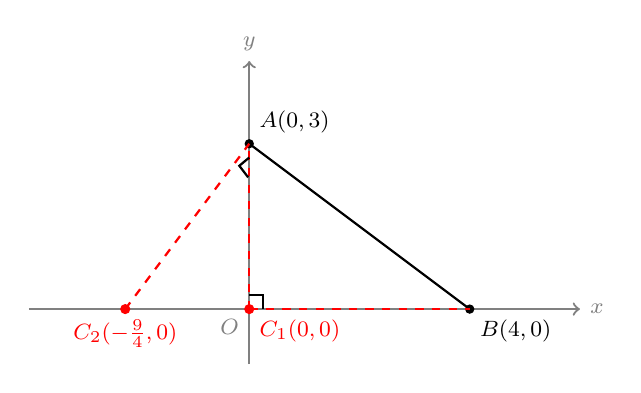
\begin{tikzpicture}[thick, scale=0.7]
  \draw[->, gray] (-4,0) -- (6,0) node[right, font=\footnotesize] {$x$};
  \draw[->, gray] (0,-1) -- (0,4.5) node[above, font=\footnotesize] {$y$};
  \node[font=\footnotesize, below left, gray] at (0,0) {$O$};
  \coordinate (A) at (0,3);
  \coordinate (B) at (4,0);
  \filldraw (A) circle (1.8pt) node[above right, font=\footnotesize] {$A(0,3)$};
  \filldraw (B) circle (1.8pt) node[below right, font=\footnotesize] {$B(4,0)$};
  \draw[thick] (A) -- (B);
  % C1 = (0,0) = O: 直角在 C
  \filldraw[red] (0,0) circle (2pt) node[red, font=\footnotesize, below right] {$C_1(0,0)$};
  \draw[red, dashed] (0,0) -- (A);
  \draw[red, dashed] (0,0) -- (B);
  % 直角标记于 C1
  \draw (0,0.25) -- (0.25,0.25) -- (0.25,0);
  % C2 = (-9/4, 0)：直角在 A
  \filldraw[red] (-2.25,0) circle (2pt) node[red, font=\footnotesize, below] {$C_2(-\frac{9}{4},0)$};
  \draw[red, dashed] (-2.25,0) -- (A);
  % 直角标记于 A: AC2 与 AB 垂直
  % AB 方向 (4,-3)，AC2 方向 (-2.25,-3)。 垂线小方块
  \draw (A) ++(0.0,-0.25) -- ++(-0.18,-0.15) -- ++(0.16,-0.21);
\end{tikzpicture}
\end{document}
